\chapter{技术路线}
\section{研究内容}
本项目旨在研究内生安全应用软件构造技术,主要研究内容是应用软件形式化建模与规约技术,为应用软件的构造提供模型和性质描述方法。
\subsection{建模}
\par
建立应用软件的形式建模是开展安全性分析、验证以及正确代码实现的基础。针对当前应用软件具有分布性、异构性、并发性和实时性等特征,研究基于状态机的应用软件行为建模方法,准确描述应用软件的控制行为和逻辑;研究基于序列图的应用软件通讯建模方法,准确描述分布式环境下应用软件的交互流程;研究开放网络环境下,应用软件运行环境、威胁、攻击的建模方法,以及用于应对威胁和攻击的信息安全策略的建模方法;研制开发应用软件安全构造集成开发套件中形式化建模模块,为应用软件的安全构造奠定基础。
\par
\subsection{规约}
\par
形式化方法的一个重要研究内容是形式规约(Formal Specification,也称形式规范或形式化描述),它是对程序“做什么”(what to do)的数学描述,是用具有精确语义的形式语言书写的程序功能描述,它是设计和编制程序的出发点,也是验证程序是否正确的依据。对形式规约通常要讨论其一 致性(自身无矛盾)和完备性(是否完全、无遗漏地刻画所要描述的对象)等性质。形式规约的方法主要可分为两类:一类是面向模型的方法也称为系统建模,该方 法通过构造系统的计算模型来刻画系统的不同行为特征;另一类是面向性质的方法也称为性质描述,该方法通过定义系统必须满足的一些性质来描述一个系统。不同 的形式规约方法要求不同的形式规约语言,即用于书写形式规约的语言(也称形式化描述语言),如代数语言OBJ、Clear、ASL、ACT One/Two等;进程代数语言CSP、CCS、π演算等;时序逻辑语言PLTL、CTL、XYZ/E、UNITY、TLA等;这些规约语言由于基于不同 的数学理论及规约方法,因而也千差万别,但它们有一个共同的特点,即每种规约语言均由基本成分和构造成分两部分构成。前者用来描述基本(原子)规约,后者 把基本部分组合成大规约。构造成分是形式规约研究和设计的重点,也是衡量规约语言优劣的主要依据。
\par
\section{研究方案}
\subsection{建模}
采用形式化建模语言、安全策略与应用软件的模型融合等关键技术对应用软件进行建模。由于应用软件具有分布性、异构性、并发性和实时性等特征,采用拓扑图和状态机相结合的方式可以准确描述应用软件的上述性质。
\par
\begin{figure}[h]
	\centering
	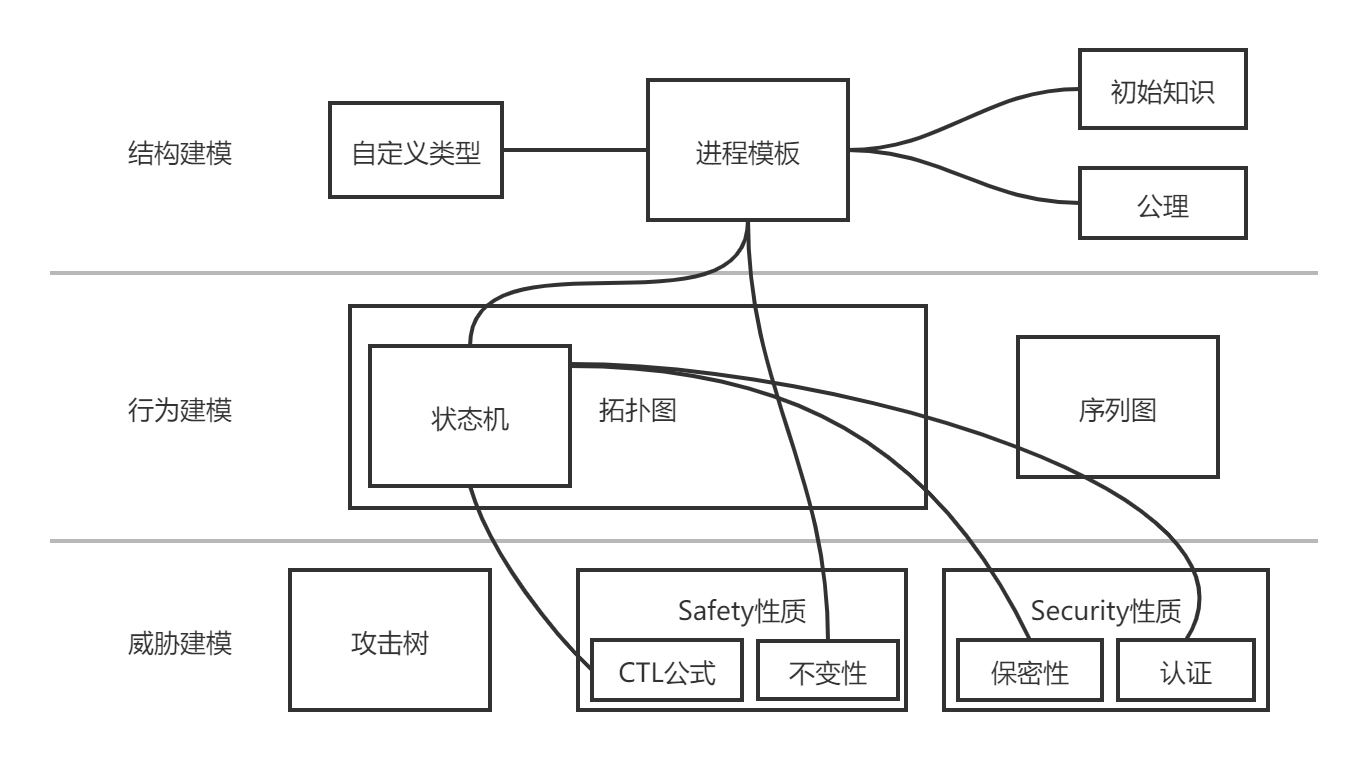
\includegraphics[width=12cm,height=6.75cm]{imgs/architecture.png}
	\caption{整体架构图}
	\label{architecture}
\end{figure}
\par
应用软件具有分布式特性,一般包括多个计算节点,单个节点进行实时计算,而节点之间通过异步消息传递来通信,因此对于分布性而言,是基于拓扑图的各个结点可以表达应用软件的不同行为。
\par
而对于异构性而言,是基于用户可以灵活架设拓扑图的二维拓扑结构;对于并发性而言,是基于拓扑图在拓扑排序上存在同层的行为结点;对于实时性而言,则要依靠拓扑图和状态机相结合的方式保证。
\par
以下将分别阐述用户建模过程中涉及的各类模型。

\subsubsection{类图建模}
类图定义了模型的静态结构,特别是模型中存在的类、类的内部结构以及它们与其他类的关系等,它是面向对象建模的重要组成部分。使用类图来对系统中涉及的各个数据结构进行建模。如网络协议中的消息包结构可使用类型嵌套的类图建模,协议的运作进程模板也将涉及程序初始变量和方法、通信方法等,同样使用相应的类图进行建模,其成分如图\ref{process}所示。
\begin{table}[h]
	\centering
	\begin{tabular}{|c|c|}
		\hline
		\textbf{成分} & \textbf{描述} \\ \hline
		Attribute           & 属性          \\ \hline
		Method              & 方法          \\ \hline
		CommMethod          & 通信手段        \\ \hline
	\end{tabular}
	\caption{进程模板类图中的成分}
	\label{process}
\end{table}

在对软件的进程模板进行建模时,还涉及进程模板的初始知识,即软件进程模板的哪些属性是软件运行初期就已知的,它也是使用类图进行建模。另外还涉及一些系统中复杂的先验知识,例如在协议中涉及到加密解密操作时,需要指明配对的加解密方法,这可以通过公理公式描述,也是使用类图进行建模。

\subsubsection{状态机建模}
状态机适合对分布式应用软件的单个节点的控制计算逻辑进行描述,在状态机的转移边上有转移条件和转移时执行的控制动作,整个状态机从初始状态到终止状态运行一遍,也就描述了软件进程从启动到结束的整个生命周期执行的行为,因此状态机建模是基于类图中进程模板的建模的。在我们的方案中,一个进程模板对应于一个状态机。同样地,对集中式的软件状态机仍然能够胜任行为建模。
\par
进程模板描述了软件对外可见的组成成分,而状态机描述了软件内部的行为,由于采用了统一语义框架的状态机和进程模板有机融合的建模语言,在状态机中可以使用进程模板暴露出的属性、方法和通信手段。以对软件执行过程中的细节进行描述。例如,网络安全协议中可以在某个状态向另一进程发送消息,而在另一状态等待消息接收并按照消息头来决定下一步的不同行为。
\par
需要注意的是,对分布式应用软件而言,将使用拓扑图描述整个软件系统。而状态机作为系统中单个结点的行为描述,也包括了分布式通信的行为,这也和进程模板本身的通信方法定义相关。总的来说,状态机在系统中将作为软件细节的重要描述手段,也是进程模板之间交互的建模中介。

\subsubsection{拓扑图建模}
拓扑图用于描述分布式软件的结点拓扑结构,对于每个结点而言,它可以选择使用已定义的进程模板,表示该结点所运行的进程。拓扑图中的不同结点可以使用不同的进程模板,也可以使用相同的进程模板,其意义即是从进程模板派生出各个具体的结点进程。
\par
由于进程模板使用唯一的状态机对其进程行为建模,所以软件的分布式结点将使用其行为作为结点的行为。但由于拓扑图中的结点还身处有向图中存在关系结构,所以其交互应具体受制于所处环境,这是拓扑图对分布式软件建模,特别是网络协议建模的重要作用。使用拓扑图用户可以构造网络中各个结点的拓扑结构,结合结点进程模板的状态机行为建模以实现对分布式网络协议的统一建模。

\subsubsection{序列图建模}
序列图是UML种的动态结构模型,用于描述执行系统功能的各个角色之间相互传递消息的顺序关系,显示对象之间的这些交互。序列图建模可以帮助用户理解和理清所建模的目标种存在哪些实体,以及他们之间的交互和信息传递顺序,也能帮助用户向其它用户传达系统流程和思想。
\par
在序列图中,主要涉及同步消息、异步消息和返回消息,其中同步消息和异步消息又可以分为到本对象的和到其它对象的。使用这样的方式可以帮助用户更好的描述系统流程中的同步和异步处理,并明确指出哪些消息是接收方对根据消息做出处理的响应,能够很好的适应网络协议建模。


\subsection{威胁和规约}
安全威胁模型是对整个攻击过程的结构化和系统化描述。开放式的网络环境以及分布式系统中应用软件的复杂特性使得对攻击模式描述越来越困难。拟研究能够对开放网络环境下应用软件多阶段安全威胁行为进行形式建模和分析的方法,研究安全策略(包括访问控制等)的形式建模方法。
\subsubsection{攻击树}
攻击树(Attack trees) 为我们提供了一种正式而条理清晰的方法来描述系统所面临的安全威胁和系统可能受到的多种攻击。我们用树型结构来表示系统面临的攻击,其中根节点代表被攻击的目标,叶节点表示达成攻击目标的方法。当攻击树应用在具体实例中时,其结构可能变得庞大而复杂。一个完整的攻击树很可能包括成百上千的叶节点,即便如此,攻击树也可以在很大程度上帮助我们判断系统存在的威胁和决定应对攻击的方法。本项目中攻击树的计算伪代码如下:
\lstset{
	caption=攻击树的计算, 
	basicstyle=\ttfamily\footnotesize,
	frame=tb,
	xleftmargin=.01\textwidth, xrightmargin=.01\textwidth
}
\begin{lstlisting}
def calculate(root):
	ans = false
	if (root.isActive):
		return calculate(root.childNodes[0])
	else:
		if root.condition == "ACTIVE":
			return calculate(root.childNodes[0])
		elif root.condition == "TRUE":
			return true
		elif root.condition == "FALSE":
			return false
		else:
			if root.name == "AND":
				ans = true
				for node in root.childNodes:
					if (!calculate(node)):
						ans = false
				return ans
			if root.name == "OR":
				ans = false
				for node in root.childNodes:
					if (calculate(node))
						ans = true
				return ans
			if root.name == "NEG":
				return !calculate(root.childNodes[0])

\end{lstlisting}
\subsubsection{安全威胁}
\par
随着集成商业应用软件部署在不同架构层的需求不断增加,反映了软件应该使用的问题。这些应用软件也必须遵循随着商业变化带来的安全需求和管理变化。此外,分布式网络也逐渐渗透在社会的各个角落和人们的日常生活中。但是,这也伴随着一些不法分子甚至敌对势力利用网络现有技术存在的缺陷来实施网络威胁行为,从而通过攻击他人的机器来获取非法利益。由于现有分布式网络威胁所日益呈现的复杂化、多步骤协同化行为特征,这对网络现有技术是严峻的挑战。在这种情况下,仅仅发现软件所忽略的漏洞的安全攻击是不够的,需要分析信息控制流问题,特别是当底层平台和基础设施也由服务本身提供时。就于这些存在的问题,我们对开放网络环境分布式软件的威胁行为的特征进行描述,刻画其行为属性,有助于了解复杂网络威胁行为,并构建相应的威胁模型和分析软件的安全属性。
\par
安全威胁分析的概念类似于权衡分析的概念,说明有多种方式来攻击系统的资产,攻击者可能同时攻击它们或者其子集。更加准确地来讲,攻击者使用特定的攻击路径或可选择的方法来达到他的攻击目的。攻击树是一种传统的方式来系统的分类系统可能被攻击的方式,威胁分析就可以由攻击树完成。攻击树是一个多层次的图,包括一个根结点,多个层次和孩子结点。另外,不同结点值可与AND,OR关系结合,从而学习更多关于系统的安全缺陷与弱点。明确地来说,攻击树的目的是来在系统规整中定义和分析潜在的攻击。结点层次与逻辑操作(例如合取(聚合)或者析取(选择)等)的形式来表示不同攻击树结点间的相互关系,从而构造这种结构。
\par
\begin{figure}[h]
	\centering
	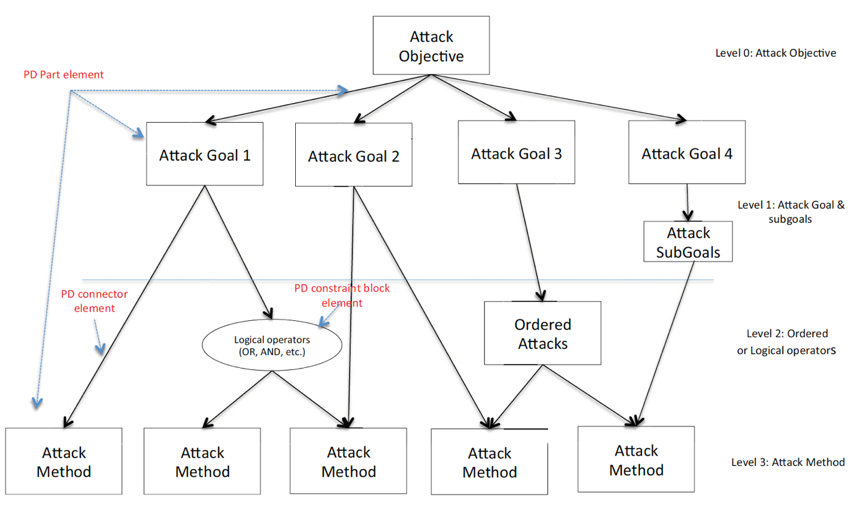
\includegraphics[width=12cm,height=6.75cm]{imgs/attacktree.png}
	\caption{Generic attack tree structure}
	\label{architecture}
\end{figure}
\par
通过使用OR操作来表示可选择的方式一个攻击者试图达到他的攻击目的。AND关系表示不同步骤来达成相同的目的。在我们的攻击树建模方法中,不仅仅考虑这两种逻辑操作,我们还考虑时序操作。特别地可以在一个攻击的攻击结点和顺序中捕获时序依赖。
\par
一个攻击树建模的整体流程如下:
\par
1、	在一个抽象的“攻击目标”上建立攻击树的根(Level0)。我们使用“Part”元素来建模各个攻击树结点。
\par
2、	它的孩子结点(Level1)表示不同的“攻击目标“来满足这次攻击目的。攻击目标和攻击目的通过一个绑定”connector”来链接。
\par
3、	对每个攻击目标结点:
\par
a)	将其分解成一系列“攻击方法”(Level 3),从而能够用来达成攻击目标
\par
b)	指定不同攻击方法之间的逻辑关系。我们使用“constraint block”来指定这些逻辑表达式。在这个阶段,我们也考虑过渡的步骤来表示某些抽象层次的攻击方法
\par
4、	当叶子条件(基本操作,让所有的细节描述攻击)达到满足攻击者的能力时,攻击树终止。
\par
我们提倡的攻击树建模方法提供了典型攻击树建模方法与反目的建模方法的桥梁。更加准确地说,攻击树建模方法的钱两步骤等驾驭KAOS反目的建模,提供了自上而下方法来建模攻击。接下去的两个步骤与标准攻击树建模方法一直,自下而上的识别攻击。
\subsubsection{安全性质规约}
\par
时序逻辑是分布式应用的一种广为接受的形式规约语言。分布式应用的功能安全性一般可以归结为系统运行轨迹的性质。时序逻辑通过几个直观的时序算子(即描述将来行为的Next和Until算子,以及描述过去行为的Previous和Since算子)的组合来方便地来描述系统运行轨迹的性质。时序逻辑一般分为线性时序逻辑和分叉时序逻辑。线性时序逻辑描述分布式系统一个运行轨迹的性质,而分叉时序逻辑描述分布式系统计算树的性质。LTL是最常用的线性时序逻辑,而CTL是最常用的分叉时序逻辑。时序逻辑还可以按照基于时间点的时序逻辑和基于区间的时序逻辑来划分,LTL和CTL都是基于时间点的时序逻辑。相对来讲,基于区间的时序逻辑一般其算法性质,比如可判定性与计算复杂性,要远远高于基于时间点的时序逻辑,从而使得对其进行推理和验证变得困难,所以基于主流的自动模型检测工具基本都采用基于时间点的时序逻辑来做为规约语言。
\par
由于线性时序逻辑可以对分布式系统的性质进行非常自然和直观的描述,我们采用线性时序逻辑及其扩展作为分布式应用的功能安全性的规约语言。安全性质,比如认证性、机密性,从本质上讲也可以归结为一条或者多条系统运行轨迹的性质。我们将分布式应用软件的信息安全性质和功能安全性质放在同一框架下进行描述。
\par
最后,我们为开发人员进行形式规约提供图形化界面支持,对于常用的一些规约模式设计可定制模版,使得开发人员可以快速准确地对一些典型安全性质进行规约。